Thuật toán tiến hóa (thuật ngữ gốc: \emph{Evolutionary Algorithm - EA})\cite{jansen2015analyzing} là tập các thuật toán được lấy cảm hứng từ ý tưởng tiến hóa \cite{darwin1859on} trong sinh học mà có thể đã khá quen thuộc với chúng ta đó là quá trình chọn lọc tự nhiên. Trong tiến hóa tự nhiên, một quần thể sẽ truyền lại những đặc tính di truyền của mình phù hợp với điều kiện sống hiện tại cho thế hệ sau. Những đặc tính này sẽ được biểu hiện và truyền lại trên gen từ bố mẹ sang con cái thông qua quá trình sinh sản. Trong đó việc các cá thể của thế hệ sau có đặc tính khác nhau là kết quả của quá trình "đột biến", "tái tổ hợp di truyền" và các "biến dị di truyền" khác. Trong quần thể, nếu một cá thể có nhiều đặc tính tốt phù hợp để sống sót với điều kiện sống nó sẽ có nhiều cơ hội để kết hợp sinh sản với các cá thể ưu tú khác trong quần thể để tạo ra những đứa con chất lượng trong thế hệ tiếp theo. Những cá thể yếu hơn và gen của chúng do không phù hợp với môi trường sống dần sẽ bị đào thải và biến mất. 

Việc mô phỏng quá trình tiến hóa tự nhiên này để phát triển một thuật toán chung nhằm dần cải thiện một cấu hình, một bộ tham số cho bất kỳ bài toán, giải pháp nào. Thuật toán bao gồm 4 bước chính như trong hình \ref{fig:ea}: khởi tạo quần thể, lựa chọn, toán tử di truyền và kết thúc. Mỗi bước sẽ tương ứng, đại khái một khía cạnh cụ thể của chọn lọc tự nhiên.

% \begin{figure}
%     \centering
%     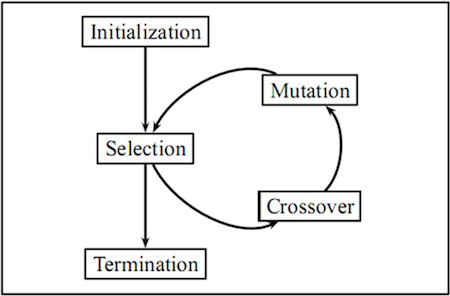
\includegraphics[width=7cm]{ea_process.jpeg}
%     \caption{Quá trình thực hiện thuật toán tiến hóa}
%     \label{fig:ea-process}
% \end{figure}

Tại mỗi thế hệ thuật toán sẽ cố gắng đưa ra một quần thể các giải pháp có chất lượng cao hơn số với thế hệ trước đó. Trong quá trình này, thuật toán sẽ thực hiện tính toán theo một thang đo phù hợp để tìm ra những cá thể có chất lượng tốt, kết hợp chúng để sinh sản ra con cái với chất lượng cao hơn tại thế hệ sau. Bởi vậy có thể coi những cá thể của thế hệ sau mang những vật liệu di truyền (gen) tốt nhất của thế hệ trước và vượt trội hơn một chút so với thế hệ trước. Hay nói một cách đơn giản, trong thuật toán tiến hóa các cá thể phù hợp sẽ tồn tại và sinh sôi nảy nở, ngược lại những cá thể yếu hơn sẽ chết đi và không đóng góp vào nhóm gen của thế hệ tiếp theo.



